% LaTeX template for a short report (written for MSES scenario modelling)
% uses LaTeX documentclass "article" for use of sections (not chapter) and References (not Bibliography)
% for Chapters and Bibliography use "documentclass "report
\documentclass[10pt]{article}   % Use article class with 10pt letter
%\documentclass[10pt]{report}
\usepackage[utf8]{inputenc}

%\usepackage[T1]{fontenc}  % 8-bit encoding, helps hyphenation of accented characters -
% https://tex.stackexchange.com/a/677/42066

% Use A4 paper and set margins:
%\usepackage[a4paper, twoside, top=2.0cm, left=3.0cm, bottom=2.0cm, right=2.0cm]{geometry}
\usepackage[a4paper, twoside, top=2.0cm, left=2.0cm, bottom=2.0cm, right=2.0cm]{geometry}
%\usepackage[a4paper, top=2.5cm, left=2.5cm, bottom=2.5cm, right=2.5cm]{geometry}

\usepackage[english]{babel}  % Hyphenation and more for English

\usepackage{pgf}      % Include graphics inside figures using \pgfimage
\usepackage[font=small, labelfont=bf]{caption}  % Stylize figure, table, etc. captions

\usepackage{parskip}         % Replace paragraph indentations with white lines
\usepackage[hyphens]{url}    % Take care of urls, e.g. wrapping in the Bibliography (hyphens: also break at -)

\usepackage{xspace}   % \xspace saves the user from having to type \  or {} after a macro name in text.

% Use the appendix package for nicer appendices:
%\usepackage[toc,page]{appendix}  % MvdS
\usepackage[titletoc]{appendix}
%\usepackage[toc,page,title]{appendix}  % Use \begin{appendices} ... \end{} iso \appendix

% \usepackage[numbib,numindex]{tocbibind}  % Add ToC, List of Figures/Tables/Code listings, Bibliography and Index to ToC
% \usepackage[]{tocbibind}       % Add ToC, List of Figures/Tables/Code listings, Bibliography and Index to ToC
\usepackage[nottoc]{tocbibind}   % ToC without extra "Contents" entry...

\usepackage{amsmath,amssymb,bbm}
\usepackage{enumerate}         % Choose alternative numberings, e.g. \begin{enumerate}[a.]

\usepackage{listings}          % Code listings
\usepackage[section, above, below]{placeins}  % \FloatBarrier - flush floats before \section by default
% \usepackage{pgf}               % Figures

\usepackage{color}
\definecolor{lightgrey}{rgb}{0.9,0.9,0.9}
\definecolor{darkgreen}{rgb}{0.0,0.6,0.0}

% Citations:

% option1: use natbib/bibtex with MvdS_number_url.bst
%\usepackage[numbers, square]{natbib}  % Use numbered citations with square brackets
%\bibliographystyle{MvdS_number_url}  % Use [1], print url = field  (plain doesn't print urls)

%option2: use biblatex/biber without *.bst file
\usepackage[backend=biber, style=numeric, citestyle=numeric-comp, sorting=none]{biblatex} 
\setlength\bibitemsep{0.5\baselineskip}
\usepackage{csquotes}

% \bibliography{mybibliography} % old-style for backward comp. in preamble for biblatex/bibtex
\addbibresource{mybibliography.bib}  % new syntax for BibLaTeX


\usepackage{fancybox}  % Use \ovalbox for key strokes

\newcommand{\ldf}{\usefont{OT1}{cmr}{m}{n}}     % Select default LaTeX font - Computer Modern Roman
%\newcommand{\ldf}{\usefont{OT1}{cmss}{m}{n}}     % Select default LaTeX font - Computer Modern Sans
%\newcommand{\ldf}{\usefont{OT1}{phv}{m}{n}}     % Select default LaTeX font - Helvetica
\newcommand{\ttbf}{\usefont{OT1}{lmtt}{bx}{n}}  % Select bold typewriter font

%\usepackage[font=sf]{caption}  % Use sans-serif font for float captions - not exactly Helvetica



\newcommand{\note}[1]{\color{red}\textbf{#1}\color{black}\xspace}
\newcommand{\marc}[1]{\color{red}\textbf{Marc: #1}\color{black}\xspace}

\newcommand{\myChapter}[1]{
  \chapter{#1}
  \minitoc  % Create a ToC of this chapter
}


% General expressions:
\newcommand{\eg}{\emph{e.g.}\xspace}
\newcommand{\ie}{\emph{i.e.}\xspace}
\newcommand{\etc}{\emph{et cetera}\xspace}
\newcommand{\ff}{\emph{ff}\xspace}

% CLI symbols:
\newcommand{\pipe}{$|$}      % Needed to avoid | in \index{}
\newcommand{\logor}{$|\,|$}  % Needed to avoid | in \index{}
\newcommand{\home}{\url{~}}  % Home directory


% Often used code names:
\newcommand{\NULL}{\code{NULL}}
\newcommand{\void}{\code{void}}
\newcommand{\stdout}{\code{stdout}}
\newcommand{\stderr}{\code{stderr}}

% Man pages:
\newcommand{\man}[2]{\texttt{man #1 #2}\xspace}
\newcommand{\mancmd}[1]{\texttt{man #1}\xspace}

% Code:
\newcommand{\prototype}[3]{\hspace*{2em}\texttt{#1} {\ttbf #2\ldf}(\texttt{#3});\xspace}  % function prototype
\newcommand{\var}[2]{\hspace*{2em}\texttt{#1} {\ttbf #2\ldf};\xspace}  % variable declaration
\newcommand{\code}[1]{\texttt{#1}\xspace}  % inline code
\newcommand{\codeb}[1]{\ttbf #1\ldf\xspace}  % inline bold code
\newcommand{\codeline}[1]{\hspace*{2em}\texttt{#1}}  % separate code line

\newcommand{\cli}[1]{\noindent\hspace*{2em}\code{\$ #1}}  % command line input
\newcommand{\clir}[1]{\noindent\hspace*{2em}\code{\# #1}}  % command line input root
\newcommand{\clo}[1]{\noindent\hspace*{2em}\code{#1}}  % command line output
\newcommand{\clitem}[1]{\item[\code{\$}] \code{#1}}  % cli in itemized list, with $ as bullet
\newcommand{\clitemb}[1]{\item[\codeb{\$}] \codeb{#1}}  % cli in itemized list, with $ as bullet - bold

\newcommand{\key}[1]{\Ovalbox{\texttt{#1}}\xspace}  % key press/combination
\newcommand{\keyb}[1]{\Ovalbox{\ttbf #1\ldf}\xspace}  % key press/combination bold


% Heat pumps
\newcommand{\COP}{\mathrm{COP}}  % COP in "math mode"
\newcommand{\COPh}{\COP_{\mathrm{heating}}}  % COP_heating in "math mode"

\newcommand{\Qh}{Q_{\mathrm{H}}}
\newcommand{\Qc}{Q_{\mathrm{C}}}
\newcommand{\Th}{T_{\mathrm{H}}}
\newcommand{\Tc}{T_{\mathrm{C}}}

\newcommand{\Tin}{T_{\mathrm{in}}}
\newcommand{\Tout}{T_{\mathrm{out}}}

\newcommand{\Ph}{P_{\mathrm{heat}}}
\newcommand{\Pheat}{P_{\mathrm{heat}}}
\newcommand{\Pc}{P_{\mathrm{cool}}}
\newcommand{\Pcool}{P_{\mathrm{cool}}}
\newcommand{\Pel}{P_{\mathrm{el}}}

\newcommand{\degr}{^\circ}
\newcommand{\tdeg}{$\degr$\xspace}
\newcommand{\degC}{\degr\mathrm{C}}
\newcommand{\tdegC}{$\degC$\xspace}

  % Custom commands

\usepackage[pdftex]{hyperref}
\hypersetup{
  colorlinks = true,  % They get a red box around them if false, better set colour to black?
  linkcolor = blue,
  filecolor = magenta,
  citecolor = blue,
  urlcolor = blue,
  % linkcolor = black,
  % citecolor = black,
  % urlcolor = black,
  pdftitle = House Model References,
  pdfauthor = Trung Nguyen,
  pdfsubject = House Models,
  pdfkeywords = house - models - Python,
  pdfcreator = TeXStudio pdfLaTeX2 on Windows,
  pdfproducer = TeXStudio pdfLaTeX2 on Windows,
  bookmarksnumbered = true,  % Number sections in PDF toc
}

\usepackage[onehalfspacing]{setspace}
\usepackage{float}

\usepackage{graphicx}
\usepackage{multirow}

%\renewcommand{\thesection}{\arabic{section}}  % needed for documentclass "report" with sections





%Document title, author and date (empty)
\title{HAN dynamic house model: Buffervessel}
\author{Maarten van den Berg\\
HAN University of Applied Sciences\\
Arnhem, The Netherlands}
% \date{}

\begin{document}
	
\ldf  % Set LaTeX default font

% Set up code listing style:
\lstset{
	language=Python,
	% Fonts:
	basicstyle=\ttfamily\footnotesize,
	%keywordstyle=\ttfamily,
	%identifierstyle=,
	%commentstyle=\ttfamily\scriptsize,
	% B/W code:
	% commentstyle=\ttfamily\itshape,  % Italic
	% stringstyle=\ttfamily,
	% identifierstyle=\ttbf,           % Bold typewriter type
	% keywordstyle=\ttbf,              % Bold tt
	% Colour:
	commentstyle=\scriptsize\ttfamily\color{brown},
	stringstyle=\ttfamily\color{darkgreen},
	identifierstyle=\color{blue},
	keywordstyle=\ttfamily\color{red},
	% Spaces:
	showstringspaces=false,
	breaklines=true,
	breakatwhitespace=true,
	% Line numbering:
	numbers=left,
	numberstyle=\tiny,
	stepnumber=2, 
	numbersep=5pt,
	% Frames:
	frame=single,
	frameround=tttt,
	backgroundcolor=\color{lightgrey},
	morekeywords={pthread_create},
}
%\renewcommand{\thelstlisting}{\thechapter.\arabic{lstlisting}}  % This is the default?
%\numberwithin{lstlisting}{section}  % AMSmath: number code listings per section
%\numberwithin{lstlisting}{chapter}  % AMSmath: number code listings per chapter

\ldf

\maketitle

%\begin{center}
%	\today
%\end{center}

\tableofcontents

\newpage

% \chapter{Introduction}

\section{Introduction}

The report give an overview and compare between the available  PID and advance python control packages. The different PID forms will be discussed in section 2. In section 3 and 4 are the most used PID python packages in practice with their advantages and disadvantages. Finally section 5 give an overview on some advance control and optimization python library.


\newpage


\section{Model description}

The model for the buffer vessel is derived from the paper of Rakesh Sinha et al. \cite{}

The model consist of a heating element, located outside of the buffer vessel, which can take water from the vessel and heat the water to a desired temperature.The hot water is then injected to the top of the buffer vessel. 

Hot water is is taken from the top of the buffer vessel on the demand side. Cooled water coming from the load is returned tot the bottom of the vessel.

A schematic description of the buffer vessel is shown below.

\begin{figure}[H]
	\centering
	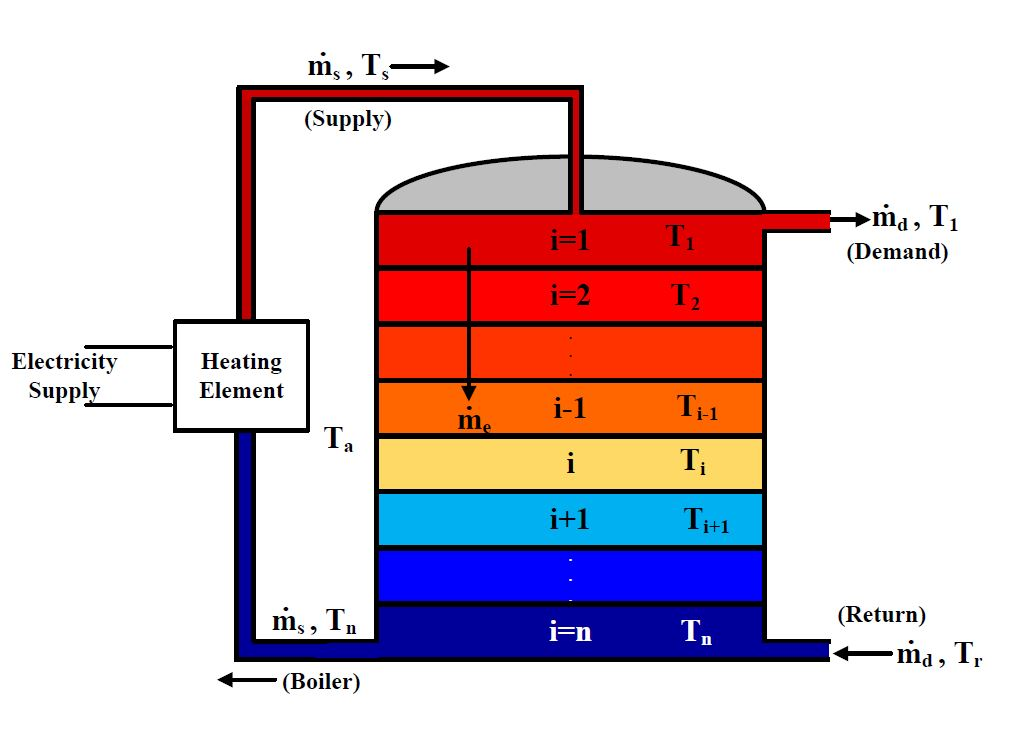
\includegraphics[width=0.8\columnwidth]{Pictures/buffervessel_setup.JPG}
	\caption[Short title]{Buffer vessel representation}
\end{figure}

Due to the fact that the density of water with different temperature layers are created.

In order to model this, the buffervessel will be divided into N-different sections 


\section{Mathematical description}


For the top layer:

\begin{equation}
	\label{eq:Buffer vessel top layer}
	mC_w \dfrac{dT_1}{dt} = \dot{m_s}C_w(T_s - T_1) + \dot{m_e}C_w(T_1 - T_2)*sgn(\dot{-m_e}) - UA_s(T_1 - T_a) - \frac{A_q\lambda_w}{z}(T_1-T_2)
\end{equation}

For the middle layers:

\begin{equation}
	\label{eq:Buffer vessel middle layers}
	mC_w \dfrac{dT_i}{dt} = \dot{m_e}C_w(T_{i-1} - T_{i})*sgn(\dot{m_e}) + \dot{m_e}C_w(T_{i} - T_{i+1})*sgn(\dot{-m_e}) - UA_s(T_i - T_a) + \frac{A_q\lambda_w}{z}(T_{i-1} + T_{i+1} - 2T_i)
\end{equation}

For the bottom layer:

\begin{equation}
	\label{eq:Buffer vessel bottom layer}
	mC_w \dfrac{dT_n}{dt} = \dot{m_d}C_w(T_r - T_n) + \dot{m_e}C_w(T_{n-1} - T_n)*sgn(\dot{m_e}) - UA_s(T_n + T_a) + \frac{A_q\lambda_w}{z}(T_{n-1}-T_n)
\end{equation}

 

\section{Validation}

To check to model from the paper, the following parameters are used:

\begin{figure}[H]
	\centering
	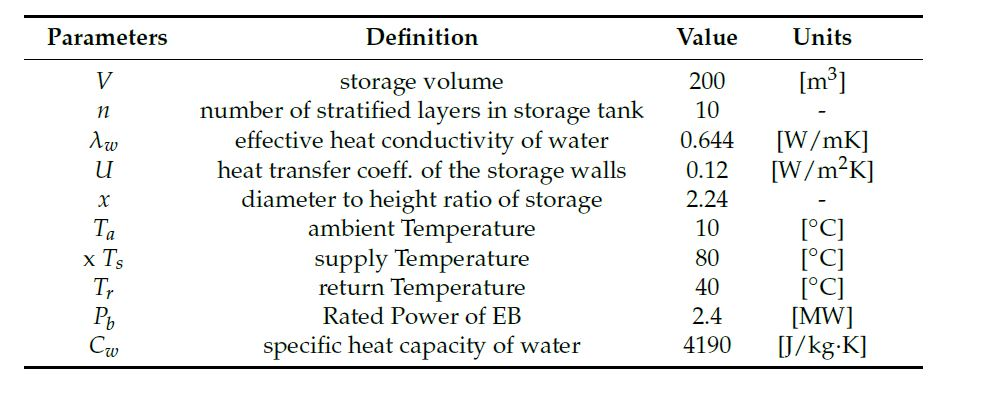
\includegraphics[width=0.8\columnwidth]{Pictures/parameters_paper.JPG}
	\caption[Short title]{Buffer vessel parameters}
\end{figure}

This results in the following graph:

\begin{figure}[H]%
	\centering
	\subfloat[\centering paper results]{{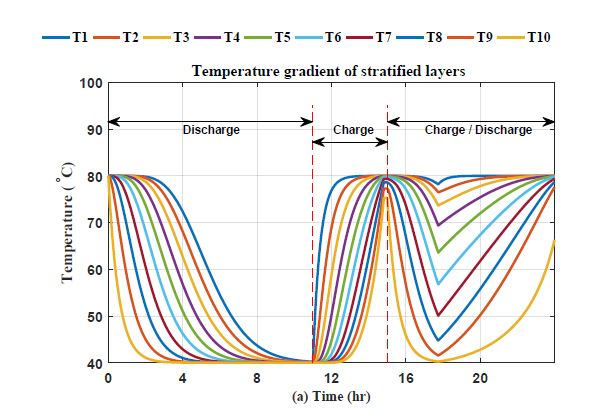
\includegraphics[width=0.8\columnwidth]{Pictures/paper_results.jpg} }}%
	\qquad
	\subfloat[\centering Python results]{{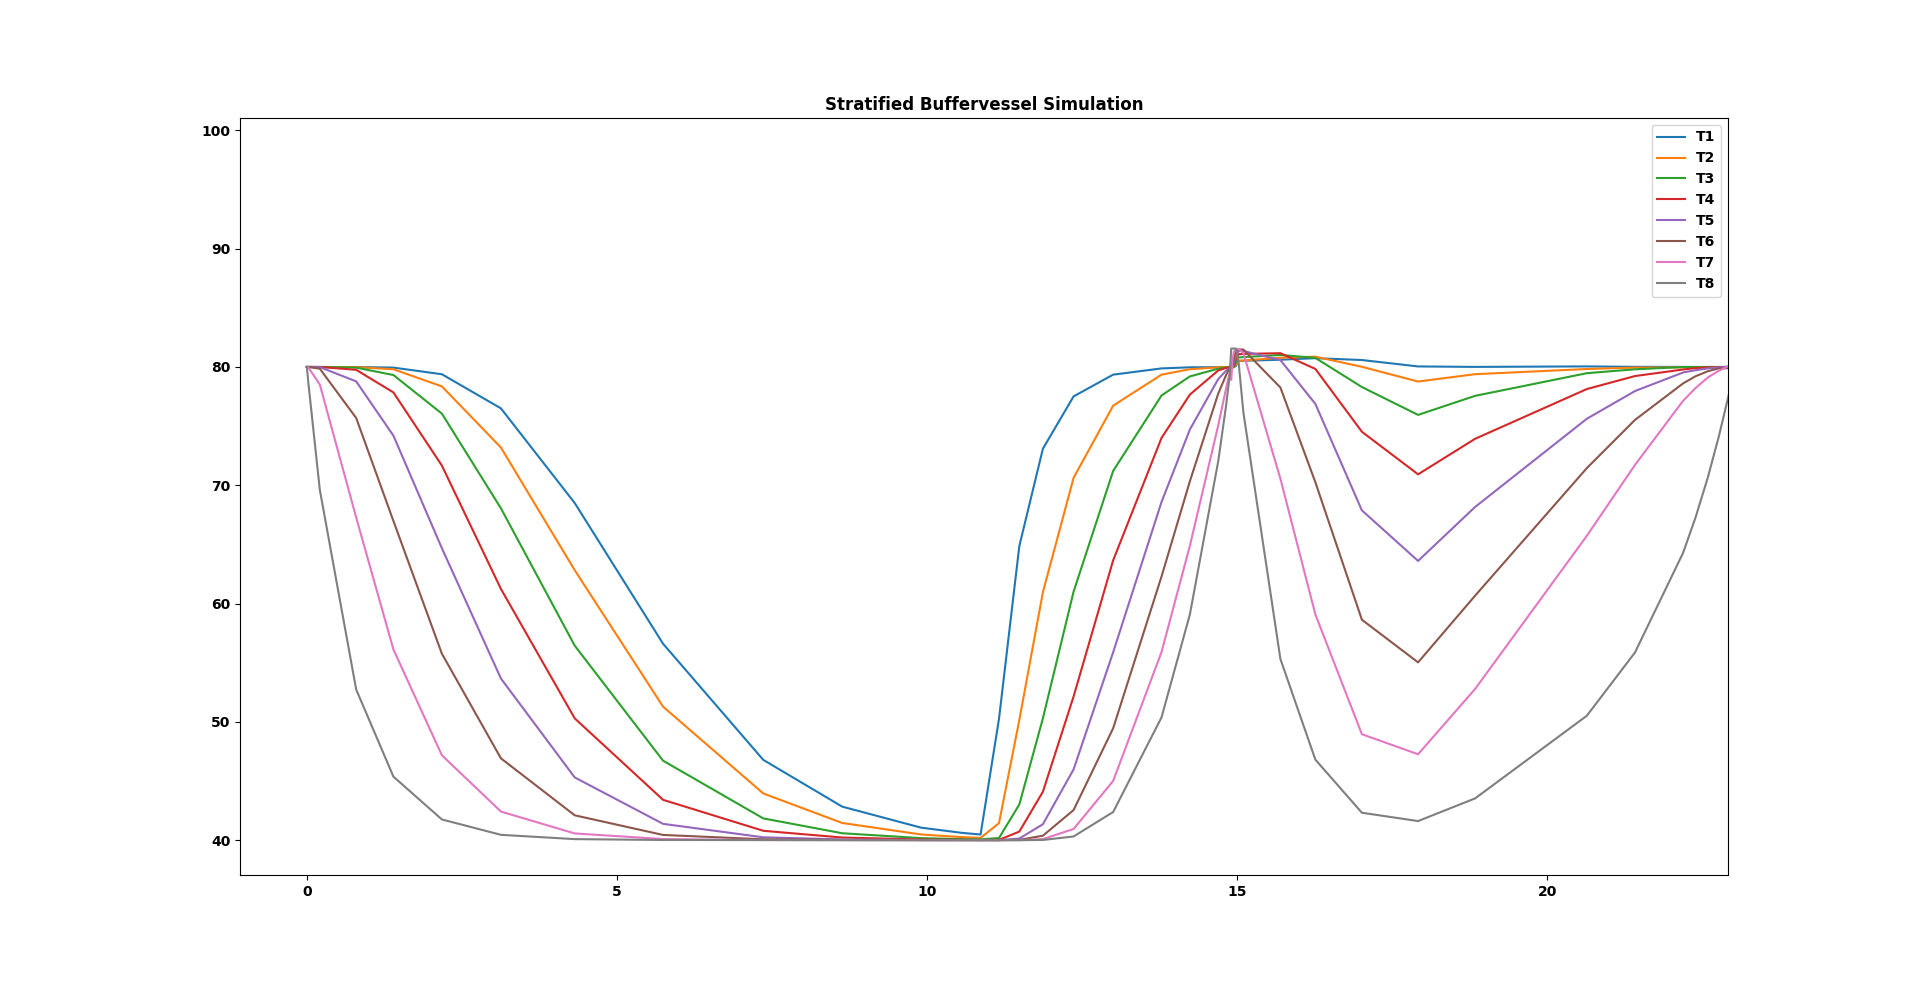
\includegraphics[width=0.8\columnwidth]{Pictures/Python_validation_graph_buffervessel.png} }}%
	\caption{Comparison between paper and python model}%
	\label{fig:Comparison}%
\end{figure}


%\bibliography{mybibliography}
\printbibliography[heading=bibintoc]

\end{document}
